\documentclass[a4paper,12pt]{book}
\usepackage{mathptmx}
\usepackage{hyperref}
\usepackage{cancel}
\usepackage{amsmath}
\usepackage{amssymb}
\usepackage{graphicx}
\usepackage{pgfplots}
\usepackage{tikz}
\usepackage{pgfplots}
\author{Gábor Hadházy and Tamás Hadházy}
\title{Mathematics}
\date{\today}

\begin{document}
\maketitle

\tableofcontents

% Chapter 1 - Algebra
\chapter{Algebra and Pre-calculus}
The first chapter is about algebra. It will cover the topics that was written by Gábor Hadházy and Tamás Hadházy. Algebra and Pre-calculus are the foundation of mathematics. It is important to understand the concepts of algebra and pre-calculus before moving on to more advanced topics.

\section{Essentials}
This section will cover the essentials in order to get started. 
\subsection{The set of Real numbers}
\begin{itemize}
    \item $\mathbb{N} = \{1, 2, 3, ...\}$ - - The set of natural numbers. 
    \item $\mathbb{Z} = \{..., -2, -1, 0, 1, 2, ...\}$ - The set of integers.
    \item $\mathbb{Q} = \{\frac{a}{b} | a, b \in \mathbb{Z}, b \neq 0\}$ - The set of rational numbers. 
    \item $\mathbb{I}$ - The set of Irrational Numbers(Real numbers that are not rational). 
    \item $\mathbb{R} = \mathbb{Q} \cup \mathbb{I}$
\end{itemize}


\subsection{The properties of Real numbers}
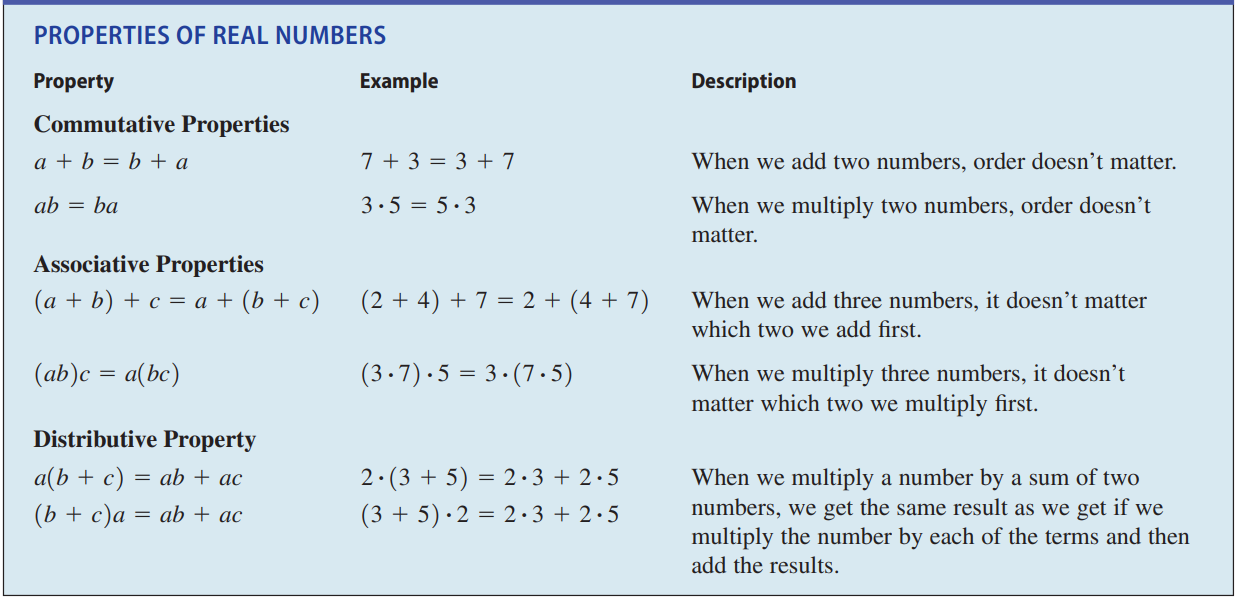
\includegraphics[width=1.1\textwidth]{algebra-pre-calculus/essentials/properties.png}

\subsection{Addition and Subtraction}
The number 0 is special for addition; it is called the additive identity because $a+0=a$ for any real number $a$. Every real number $a$ has a negative, $-a$, that satisfies $a+(-a)=0$. Subtraction is the operation that undoes addition; to subtract a number from another, we simply add the negative of that number. By definition
$$
a-b=a+(-b)
$$
To combine real numbers involving negatives, we use the following properties.
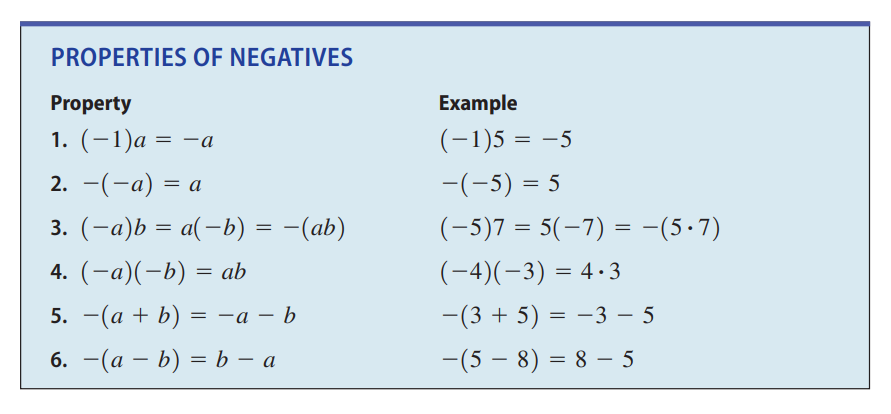
\includegraphics[width=1.1\textwidth]{algebra-pre-calculus/essentials/properties_addition_subtraction.png}

Property 6 states the intuitive fact that $a-b$ and $b-a$ are negatives of each other. \\
Property 5 is often used with more than two terms:
$$
    -(a+b+c)=-a-b-c
$$

\subsection{Multiplication and Division}
The number 1 is special for multiplication; it is called the \textbf{multiplicative identity} because $a \cdot 1=a$ for any real number $a$. Every nonzero real number $a$ has an inverse, $1 / a$, that satisfies $a \cdot(1 / a)=1$. Division is the operation that undoes multiplication; to divide by a number, we multiply by the inverse of that number. If $b \neq 0$, then, by definition,
$$
a \div b=a \cdot \frac{1}{b}
$$
We write $a \cdot(1 / b)$ as simply $a / b$. We refer to $a / b$ as the quotient of $a$ and $b$ or as the fraction $a$ over $b$; $a$ is the numerator and $b$ is the denominator (or divisor). To combine real numbers using the operation of division, we use the following properties. \\
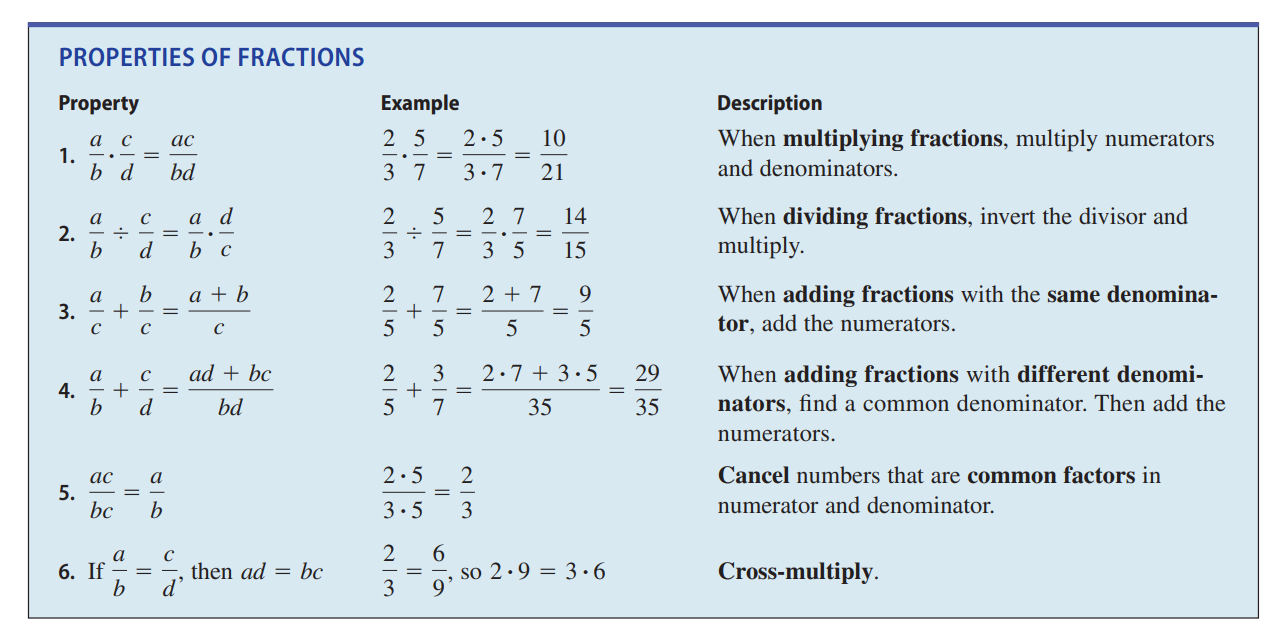
\includegraphics[width=1.1\textwidth]{algebra-pre-calculus/essentials/properties_multiplication_division.png}

When adding fractions with different denominators, we don’t usually use Property 4.
Instead we rewrite the fractions so that they have the smallest possible common denominator (often smaller than the product of the denominators), and then we use Property 3. This
denominator is the Least Common Denominator (LCD) described in the next example.

\subsection{Using the LCD to Add Fractions}

Evaluate: $\frac{5}{36}+\frac{7}{120}$
\textbf{Solution.} Factoring each denominator into prime factors gives
$$
36=2^2 \cdot 3^2 \quad \text { and } \quad 120=2^3 \cdot 3 \cdot 5
$$
We find the least common denominator (LCD) by forming the product of all the prime factors that occur in these factorizations, using the highest power of each prime factor. Thus the LCD is $2^3 \cdot 3^2 \cdot 5=360$. So
$$
\begin{aligned}
\frac{5}{36}+\frac{7}{120} & =\frac{5 \cdot 10}{36 \cdot 10}+\frac{7 \cdot 3}{120 \cdot 3} & \text { Use common denominator } \\
& =\frac{50}{360}+\frac{21}{360}=\frac{71}{360} & \begin{array}{l}
\text { Property } 3: \text { Adding fractions with the } \\
\text { same denominator }
\end{array}
\end{aligned}
$$

\subsection{Real line}

The real numbers can be represented by points on a line, as shown below. The
positive direction (toward the right) is indicated by an arrow. We choose an arbitrary
reference point O, called the origin, which corresponds to the real number 0. Given any
convenient unit of measurement, each positive number x is represented by the point on
the line a distance of x units to the right of the origin, and each negative number -x is
represented by the point x units to the left of the origin. The number associated with the
point P is called the coordinate of P, and the line is then called a coordinate line, or a
real number line, or simply a real line. Often we identify the point with its coordinate
and think of a number as being a point on the real line.

\begin{align*}
    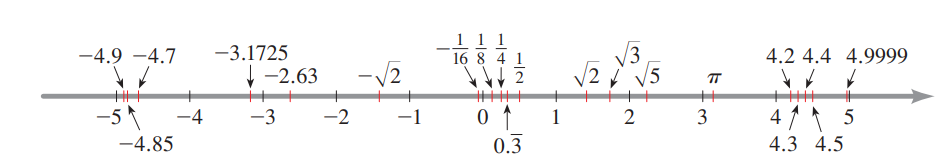
\includegraphics[width=1.1\textwidth]{algebra-pre-calculus/essentials/real-line.png}
\end{align*}

\section{Absolute Value and Distance}
The absolute value of a number $a$, denoted by $|a|$ , is the distance from $a$ to 0 on
the number line. Distance is always positive or zero, so we have
$|a|\geq0$ for every number $a$. Remembering that $-a$ is positive when $a$ is negative, we have the following definition.

\begin{equation*}
    |a| = \begin{cases}
        \;a  & \textnormal{if} \ a \geq 0 \\
        \;-a & \textnormal{if} \ a < 0
    \end{cases}
\end{equation*}

(a) $|3|=3$ \\
(b) $|-3|=-(-3)=3$ \\
(c) $|0|=0$ \\
(d) $|3-\pi|=-(3-\pi)=\pi-3 \quad($ since $3<\pi \quad \Rightarrow \quad 3-\pi<0)$

\subsection{Properties of Absolute Value}
\begin{enumerate}
    \item $|a| \geq 0$
    \item $|a|=|-a|$
    \item $|a b|=|a||b|$
    \item $\displaystyle \left|\frac{a}{b}\right|=\frac{|a|}{|b|}$
    \item $|a+b| \leq|a|+|b|$
\end{enumerate}

\subsection{Distance Between Points on the Real line}

What is the distance on the real line between the numbers -2 and 11? From
Figure 11 we see that the distance is 13. We arrive at this by finding either
$ |11-(-2)|=13$ or $|(-2)-11=13|$. From this observation we make the following definition. \\

If $a$ and $b$ are real numbers, then the \textbf{distance} between the points $a$ and $b$ on the real line is: \\
$$ d(a,b)=|a-b| $$

From the Property 6 of negatives it follows that
$$ |b-a| = |a-b|$$
$$ |3-7| = |7-3| = 4 $$

This confirms that, as we would expect, the distance from a to b is the same as the
distance from b to a.

\textbf{Example.} The distance between then numbers -8 and 2 is $d(-8,2)=|-8-2|=|-10|=10$.

\subsubsection*{Exercises}
For Exercises please download the book from here(\url{https://faculty.ksu.edu.sa/sites/default/files/precalculus-mathematics_for_calculus-j._stewart_l._redlin_and_s._watson-cengage_learning_7th_edition_2015.pdf}) and you can go to the 37th page for exercises.  % Section 1 - Essentials
\section{Exponentiation}
When starting out with Exponentiation it is important first to understand the different parts of an exponential expression, so let's consider:
$$b^x = \underbrace{b \cdot b \cdot ... \cdot b}_{x \ times}$$
\begin{itemize}
  \item $b$ is the \textbf{base}.
  \item $x$ is the \textbf{exponent}.
\end{itemize}

As a reminder $ x^0 = 1 $

Let's discuss the different rules of Exponentiation:
\subsection{Product Rule}
To find the product of two exponential expression with the same base, add the exponents. 
$$ x^{n} \cdot x^{m} = x^{n+m} $$

\subsection{Quotient Rule}
When two exponential expressions with the same base are divided,  to find their quotient subtract their exponents. 
$$ \frac{x^n}{x^m} = x^{n-m} $$

\subsection{Power Rule}
When you raise an power to a power in an exponential expression to get the product, multiply the exponents
$$ (x^{n})^{m} = x^{n \cdot m} $$ 
$$ OR $$
$$ (x^{n})^{m} = \underbrace{x^n \cdot ... \cdot x^n}_{m \ times} $$
Here it is proven that the power rule is simply just the product rule.

\subsection{Negative Exponents}
When dealing with negative exponents this equation will apply: 
$$ x^{-n} = \frac{1}{x^n} $$

Since, 
$$ \frac{1}{x} = \frac{x^0}{x^1} = x^{0-1} = x^{-1} $$
It is important to note that this is just only one way of proving this, there are a couple more. 

\subsection{Fractional Exponents}
$$ \large x^{\frac{1}{n}} = \sqrt[n]{x} $$
The proof of this can be found in the next section \hyperref[sec:radicals]{Radicals(click to redirect)}.

\subsection{Additional rules}
Distribute an exponent over a product: $(x \ y)^{n} = x^{n} \ y^{n}$ \\
Distribute an exponent over a quotient: $  (\frac{a}{b})^{n} = \frac{a^{n}}{b^{n}}$

\begin{align*}
  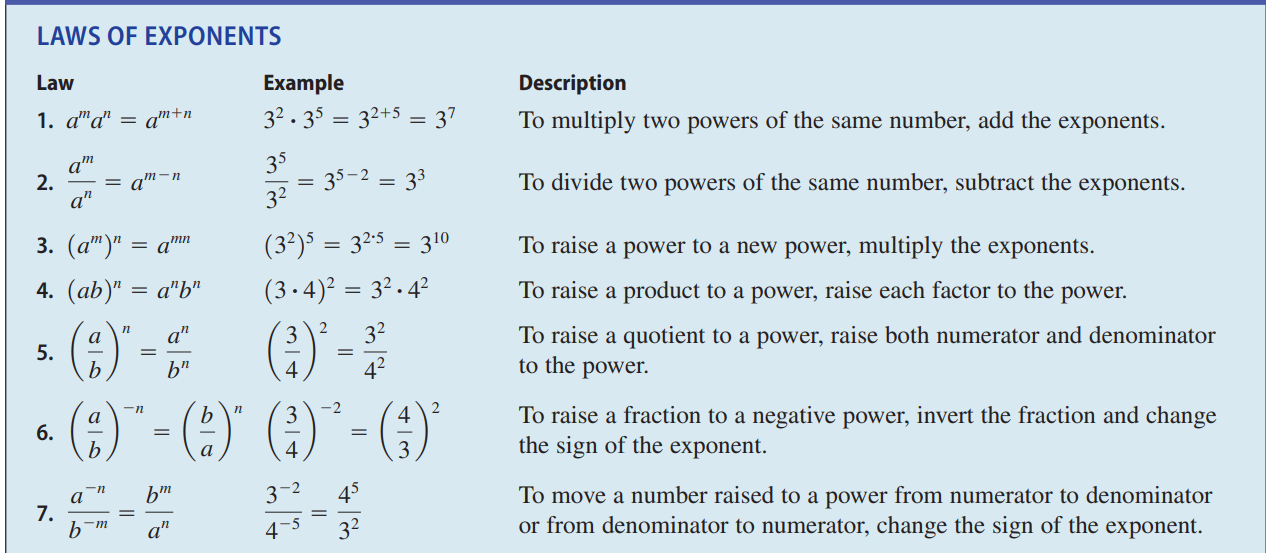
\includegraphics[width=1.2\textwidth]{algebra-pre-calculus/exponentiation/laws-of-exponents.png}
\end{align*}

\newpage % Section 2 - Exponentiation
\label{sec:radicals}
\section{Radicals}
$$ \large \sqrt[n]{x} $$
\begin{itemize}
  \item $x$ is the \textbf{radicand}.
  \item $n$ is the \textbf{index}(nth root).
  \item $\large \sqrt[n]{x}$ expression is the \textbf{radical}
\end{itemize}

As promised let's look at the fractional exponent equation. If $n$ is a positive integer that is greater than $1$ and a is a real number then,
$$ \sqrt[n]{a} = a^{\frac{1}{n}} $$

We are often referring the left side of the equation as the \textbf{radical form} and the right side of the equation as the \textbf{exponent form}

\subsubsection{Proof}
In order to prove this equation we can establish first this: 
$$ (a^{\frac{1}{n}})^{n} = a^{n \cdot \frac{1}{n}} = a^{\frac{n}{n}} = a $$
Let's take an example to avoid confusion: 
$$ (9^{\frac{1}{2}})^2 = 9^{\frac{1}{2} \cdot2} = 9^{\frac{2}{2}} = 9 $$

To put this into words $ 9^{\frac{1}{2}} $ is the number that when squared will return back $ 9 $. In other words this is exactly what it meant by the root(in this case square root) which will return back the number that when squared it will be 9. Therefore: 
$$ 9^{\frac{1}{2}} =  \sqrt[2]{9} = 3 $$

Since,
$$ (3)^2 = 9 = (9^{\frac{1}{2}})^2 $$

Therefore the equation has been proven: 
$$ \sqrt[n]{a} = a^{\frac{1}{n}} $$

It is very important to note a misconception here. The index is required in these radical expressions to make sure that we correctly evaluate the radical. There is one exception to this rule and that is square root.
$$ \sqrt[2]{a} = \sqrt[]{a} $$
In every other cases we \textbf{must} define the index, because otherwise it will be considered as a square root, Whenever working with square roots the index can be omitted.

\subsubsection{General rational exponent}
Since, $ a^{\frac{1}{n}} = \sqrt[n]{a} $.
Let's establish the general rational exponent in terms of radicals as follows. 
$$ a^{\frac{m}{n}} = (a^{\frac{1}{n}}) ^{m} = (\sqrt[n]{a})^m $$
$$ OR $$
$$ a^{\frac{m}{n}} = (a^m) ^{\frac{1}{n}} = \sqrt[n]{a^m} $$

Since being aware of the \textbf{Associative Property of Multiplication}, the order of the multiplication can be changed. 

Therefore, 
$$ a^{\frac{m}{n}} = \sqrt[n]{a^m} $$

\subsection{Properties of radicals}
\begin{itemize}
  \item $\sqrt[n]{a^n} = a$ \ This is simply true because when trying to find the $n$th root of a number and  also raising the number to that power then that's simply will be equal to the number.  \\
Consider this as an example,
$$ \sqrt[]{9^2} = \sqrt[]{81} = 9$$
   \item $ \sqrt[n]{ab} = \sqrt[n]{a} \sqrt[n]{b} $ \\
   To prove this consider this, \\
    1. Start with the left-hand side (LHS) of the equation,
    $ \sqrt[n]{ab} $ Using the definition of the nth root:
    $ \sqrt[n]{ab} = (ab)^{\frac{1}{n}} $ \\
    2. Next apply the product rule of exponents, which states that $ a^m \cdot a^n = a^{m+n} $ Therefore, $ (ab)^{\frac{1}{n}} = a^{\frac{1}{n}} \cdot b^{\frac{1}{n}} $ \\ 
    3. Now, rewrite the exponents as radicals:
    $ a^{\frac{1}{n}} $ is equivalent to $ \sqrt[n]{a} $ and $ b^{\frac{1}{n}} $ is equivalent to $ \sqrt[n]{b} $ \\
    4. So, we have: $ a^{\frac{1}{n}} \cdot b^{\frac{1}{n}} = \sqrt[n]{a} \cdot \sqrt[n]{b} $ \\
    5. Finally this proves that: $ \sqrt[n]{ab} = \sqrt[n]{a} \cdot \sqrt[n]{b} $
    \item $ \large \sqrt[n]{\frac{a}{b}} = \frac{\sqrt[n]{a}}{\sqrt[n]{b}} $ To prove this consider this, \\
    1. As previously Start with the left-hand side (LHS) of the equation: $ \sqrt[n]{\frac{a}{b}} $ \\
    2. Now using the definition of the nth root: $ \sqrt[n]{\frac{a}{b}} = \left(\frac{a}{b}\right)^{\frac{1}{n}} $ \\
    3. Apply the power rule of the exponents which states that: \\ $ (a^m)^{\frac{1}{n}} = a^{m \cdot \frac{1}{n}} = a^{\frac{m}{n}}$, Therefore when we are dealing with a fraction as the base it is the same when dealing with numbers that are not fractions: 
$$ \left(\frac{a}{b}\right)^{\frac{1}{n}} = \frac{a^{\frac{1}{n}}}{b^{\frac{1}{n}}} $$ Since, \\
$$ (\frac{a}{b})^c = \frac{a^c}{b^c} $$ \\
With an example: $ (\frac{a}{b})^2 = \frac{a}{b} \cdot \frac{a}{b} = \frac{a^2}{b^2} $ \\
	4. Now rewrite the exponents as radicals: $ a^{\frac{1}{n}} $ is equivalent to $ \sqrt[n]{a} $ and  $b^{\frac{1}{n}}$ is equivalent to $ \sqrt[n]{b} $ \\
	5. So, we have: 
	$$ \frac{a^{\frac{1}{n}}}{b^{\frac{1}{n}}} = \frac{\sqrt[n]{a}}{\sqrt[n]{b}} $$ \\
	6. Finally, this proves that: 
	$$ \sqrt[n]{\frac{a}{b}} = \frac{\sqrt[n]{a}}{\sqrt[n]{b}} $$ \\
	\\
	
	\item Also note that while we can “break up” products and quotients under a radical we can’t do the same thing for sums or differences. In other words,
	$$ \sqrt[n]{a+b} \neq \sqrt[n]{a}+ \sqrt[n]{b}  $$ 
	$$ AND $$
	$$ \sqrt[n]{a-b} \neq \sqrt[n]{a}- \sqrt[n]{b} $$ \\
These can simply be proven by examples, 
$$ 5 = \sqrt25 = \sqrt{9+16} \neq \sqrt9 + \sqrt16 = 3+4 = 7 $$

\end{itemize} % Section 3 - Radicals
\section{Algebraic Expressions}
A \textbf{variable} is a letter that can represent any number from a given set of numbers. If we
start with variables, such as $x$, $y$, and $z$, and some real numbers and combine them using
addition, subtraction, multiplication, division, powers, and roots, we obtain an \textbf{algebraic expression}. Here are some examples:

$$ 
    2x^2-3x+4 \quad \sqrt{x}+10 \quad \frac{y-2z}{y^2+4}
$$

A \textbf{monomial} is an expression of the form $ax^k$
, where a is a real number and k is a
nonnegative integer. A \textbf{binomial} is a sum of two monomials and a \textbf{trinomial} is a sum
of three monomials. In general, a sum of monomials is called a \textbf{polynomial}. For example, the first expression listed above is a polynomial, but the other two are not.

\begin{align*}
    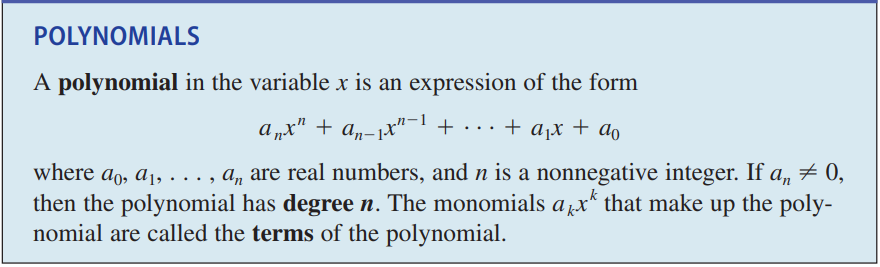
\includegraphics[width=1.1\textwidth]{algebra-pre-calculus/algebraic-expressions/polynomial definition.png}
\end{align*} \break

Note that the degree of a polynomial is the highest power of the variable that appears
in the polynomial.


\begin{align*}
    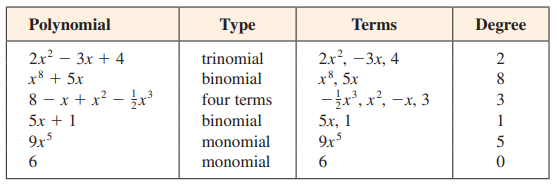
\includegraphics[width=1.1\textwidth]{algebra-pre-calculus/algebraic-expressions/algebraic-expression-spreadsheet.png}
\end{align*} \break

We add and subtract polynomials using the properties of real numbers that were discussed earlier. The idea is to combine like terms (that is, terms with the same
variables raised to the same powers) using the Distributive Property. For instance,

$$ 
    5x^7+3x^7-2x^7 = (5+3-2)x^7 = 6x^7
$$

But we already know this. 

To find the product of polynomials or other algebraic expressions, we need to use the
Distributive Property repeatedly. In particular, using it three times on the product of two
binomials, we get

$$ 
    (a+b)(c+d) = a(c+d)+b(c+d) = ac+ad+bc+bd
$$

\subsection{Special Product Formulas}
Certain types of products occur so frequently that you should memorize them. You can
verify the following formulas by performing the multiplications.

\begin{align*}
    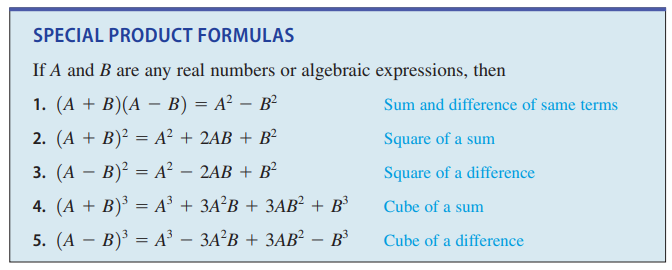
\includegraphics[width=1.1\textwidth]{algebra-pre-calculus/algebraic-expressions/special_product_formulas.png}
\end{align*} \break

\subsection{Factoring Common Factors}
We use the Distributive Property to expand algebraic expressions. We sometimes need
to reverse this process (again using the Distributive Property) by factoring an expression as a product of simpler ones.
For example,
\begin{align*}
    &A. \quad 15 + 25x = 5(3 + 5x) \\
    &B. \quad x^2y + y^2x^3 = x^2y(1 + xy) \\
\end{align*}
You can always check whether you have factored correctly by expanding the brackets.

\subsection{Factoring quadratics}
A quadratic is an expression with a squared term, then just a term with a variable, then a constant. 
\\ Like this: $ax^2 + bx + c$ 
More about solving quadratic equations and quadratic equations in general can be found in the next section \hyperref[sec:quadratic-equations]{Quadratic Equations(click to redirect)}.


We are looking for two numbers that multiply you get $c$ and when you add them you get $b$.
The reason why: 
$$ (x + m)(x + n) = \\ x^2 + mx + nx + mn = x^2 + \underbrace{(m + n)}_b x + \underbrace{(mn)}_c $$

$m$ and $n$ are the two numbers we are looking for. As you can see $m + n = b$ and $mn = c$. \\

\textbf{Example}. Factor $x^2 - 6x + 8$ \\
We are looking for two numbers that multiply you get $8$ and when you add them you get $-6$. \\
The two numbers are $-2$ and $-4$ because $-2 \cdot -4 = 8$ and $-2 + -4 = -6$. \\
Therefore, 
\begin{align*}
    x^2 - 6x + 8 &= (x - 2)(x - 4) \\
\end{align*}

\textbf{Example}. Factor $10x^2 + 11x - 6$ \\
\begin{itemize}
    \item Step 1. Multiply the leading coefficient (10) and the constant term (-6) to get -60. \\
    \textbf{Why?} The main goal in factoring a quadratic equation is to express it as the product of two binomials(like (2x+4)(4x+5)). 
    In the case of a quadratic with a leading coefficient (the coefficient of $x^2$) not equal to 1, like $10x^2$ in our example, we need to find two binomials of the form $(ax + b)(cx + d)$ e.g $(2x + 4)(5x+2)$ such that their product equals the given quadratic. 
    So, in this context, we are essentially trying to break down the original quadratic ($10x^2 - 11x - 6$) into two binomials, and we start by looking for two numbers that will help us achieve this. These two numbers should meet two criteria:
    \begin{itemize}
        \item Their product should equal the product of the leading coefficient and the constant term (in this case, $10 \cdot -6 = -60$).
        \item Their sum should equal the coefficient of the x-term (in this case, -11)
    \end{itemize}
    By finding such numbers, we can rewrite the middle term of the quadratic equation (the -11x term) as the sum or difference of two terms, each of which can be factored more easily. This allows us to perform factoring by grouping, making the overall factoring process more manageable.
    \item Step 2.  Find two numbers that multiply to -60 and add up to the coefficient of the x-term (-11). In this case, those two numbers are -15 and 4 because $(-15) \cdot 4 = -60$ and $(-15) + 4 = -11$.
    \item Step 3. Rewrite the middle term (-11x) using the two numbers found in step 2: 
    $$ 10x^2 - 15x + 4x - 6 $$
    \item Step 4. Group the terms: Group the first two terms $(10x^2 - 15x)$ and the last two terms $(4x - 6)$. This will gve us: 
    $$ 5x(2x - 3) + 2(2x - 3) $$
    \item Step 5. Factor out the HCF of each group: 
    $$ 5x(2x - 3) + 2(2x - 3) = (5x + 2)(2x - 3) $$

\end{itemize}
And we are done factorising the quadratic equation.

\subsection{Difference of squares}
The difference of squares is a squared term minus another squared term.
\\ Like this: $a^2 - b^2 = (a+b)(a-b) = a^2-ab+ab-b^2 $ 

\textbf{Example.} Factor $x^2 - 9$ 
$$ (x+3)(x-3) $$


\textbf{Example.} Factor $9p^2 - 1$ 
$$ (3p+1)(3p-1) $$

\subsection{Difference or sum of cubes}
The difference or sum of cubes is a cubed term plus or minus another cubed term.

$$ a^3 - b^3 = (a-b)(a^2+ab+b^2) $$ Because, $$(a-b)(a^2+ab+b^2) = a^3 - ab^2 + a^2b - ab^2 + b^3 = a^3 - 2ab^2 + b^3 $$ 

And, 
$$ a^3 + b^3 = (a+b)(a^2-ab+b^2) $$ Because, $$(a+b)(a^2-ab+b^2) = a^3 + ab^2 - a^2b + ab^2 + b^3 = a^3 + 2ab^2 + b^3 $$ 
\\
\textbf{Example.} Factor $x^3 - 8$ \\
We know that $x^3 - 8 = x^3 - 2^3$
Therefore,
$$ (x-2)(x^2+2x+4) $$

if we expand out: 
$$ (x-2)(x^2+2x+4) = x^3 + 2x^2 + 4x - 2x^2 - 4x - 8 = x^3 - 8 $$
Therefore our answer is correct.

\subsection{Additional examples of factoring}
\textbf{Example.} Which of these expressions DOES NOT factorise?

A. $x^2 + x$ \\
This can be factored by pulling out the highest common factor. \\
$$ x^2 + x = x(x+1) $$

B. $x^2 - 25$ \\
This also can be factored by difference of squares. \\
$$ x^2 - 25 = (x+5)(x-5) $$

C. $x^2 + 4$ \\
This cannot be factored because it is a sum of squares not a difference of squares. \\

D. $x^3+2x^2+3x+6$ \\
This can also be factored by grouping. \\
$$ x^3+2x^2+3x+6 = x^2(x+2)+3(x+2) = (x^2+3)(x+2) $$

E. $5x^2-14x+8$ \\
This can also be factored by using the method of factoring quadratics when $a \neq 1$. \\
Therefore we can multiply the leading coefficient (5) and the constant term (8) to get 40. \\
We are looking for two numbers that multiply you get 40 and when you add them you get -14 and those are -10 and -4. \\
So we can rewrite the middle term (-14x) using the two numbers found:
$$ 5x^2 - 10x - 4x + 8 $$ 
Then we can group them together:
$$ 5x(x - 2) - 4(x - 2) $$
And finally factor out the HCF of each group:
$$ (5x - 4)(x - 2) $$

Eventually the answer for our question is C. $x^2 + 4$ because it cannot be factored.

\subsection{Tips and Extra examples}
\begin{itemize}
    \item Always look for the highest common factor first. That will simplify things and make the rest of the factoring more easier. 
    \item You might need to do several steps of factoring to get the final answer. For example you might have to pull out the HCF first then you can do factoring by grouping or factoring quadratics. Then you might also apply difference of squares or difference or sum of cubes. Keep factoring as far as you can go.
\end{itemize}

\textbf{Extra Example} Factor $2z^2 + 3z -14$ \\
Again as previously done first we need to multiply the leading coefficient (2) and the constant term (-14) to get -28. \\ 
We are looking for two numbers that multiply you get -28 and when you add them you get 3 and those are 7 and -4. \\
So we can rewrite the middle term (3z) using the two numbers found:
$$ 2z^2 + 7z - 4z - 14 $$ 
Then we can group them together:
$$ z(2z + 7) - 2(2z + 7) $$
And finally factor out the HCF of each group:
$$ (z - 2)(2z + 7) $$

\textbf{Extra Example} Factor $-5v^2-45v+50$ \\
Again as previously done first we need to multiply the leading coefficient (-5) and the constant term (50) to get -250. \\
We are looking for two numbers that multiply you get -250 and when you add them you get -45 and those are -50 and 5. \\
So we can rewrite the middle term (-45v) using the two numbers found:
$$ -5v^2 - 50v + 5v + 50 $$ 
Then we can group them together:
$$ -5v(v + 10) + 5(v + 10) $$
And finally factor out the HCF of each group:
$$ (-5v + 5)(v + 10) $$
This can be further simplified to:
$$ -5(v - 1)(v + 10) $$
Another solution for this could have been that first we could have pulled out the HCF which is -5 and then we could have factored the quadratic. \\
$$ -5v^2 - 45v + 50 = -5(v^2 + 9v - 10) $$
And this is really easy since $ a = 1 $ Therefore we need two numbers that multiply you get -10 and when you add them you get 9 and those are 10 and -1. \\
So we can say that: 
$$ -5(v^2 + 9v - 10) = -5(v + 10)(v - 1) $$

\subsection{Special Factoring Formulas}
\begin{align*}
    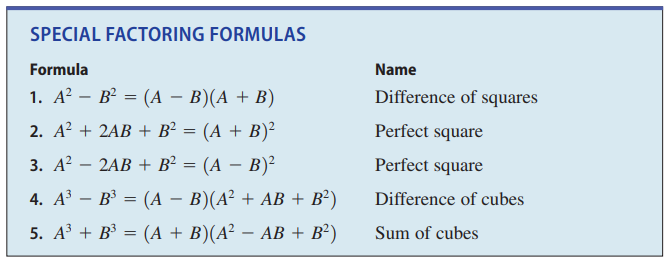
\includegraphics[width=1.1\textwidth]{algebra-pre-calculus/algebraic-expressions/special_factoring_formulas.png}
\end{align*} \break

When we factor an expression, the result can sometimes be factored further. In general, we first factor out common factors, then inspect the result to see whether it can be
factored by any of the other methods of this section. We repeat this process until we
have factored the expression completely

\subsection{Factoring Expressions with Fractional Exponents}
Factor each expresson. \\ \break
\textbf{(a)} \scalebox{1.2}{$3x^{\frac{3}{2}}-9x^{\frac{1}{2}}+6x^{-\frac{1}{2}}$ = $3x^{-\frac{1}{2}}(x^2-3x+2)$ = $3x^{-\frac{1}{2}}(x-2)(x-1)$} \\ \break
Here we have taken the common factor $3x^{-\frac{1}{2}}$ out of each term. Then we have factored the quadratic expression $x^2-3x+2$. \\ \break

\textbf{(b)} $(2+x)^{-\frac{2}{3}}x+(2+x)^{\frac{1}{3}} = (2+x)^{-\frac{2}{3}}[x+(2+x)] = (2+x)^{-\frac{2}{3}}(x+2+x) = (2+x)^{-\frac{2}{3}}(2x+2)$ \\ \break
Here we have taken the common factor $(2+x)^{-\frac{2}{3}}$ out of each term. Then we have just simplified. \\ \break % Section 4 - Algebraic Expressions
\section{Rational Expressions}
A quotient of two algebraic expressions is called a \textbf{fractional expression}. Here are
some examples:
$$ \frac{2x}{x-1} \quad \frac{y-2}{y^2+4} \quad \frac{x^3-x}{x^2+5x+6} \quad \frac{x}{\sqrt{x^2+1}}$$

A \textbf{rational expression} is a fractional expression in which both the numerator and the
denominator are polynomials. For example, the first three expressions in the above
list are rational expressions, but the fourth is not, since its denominator contains a
radical. In this section we learn how to perform algebraic operations on rational expressions.

\subsection{The Domain fo an Algebraic Expression}
In general, an algebraic expression may not be defined for all values of the variable.
The \textbf{domain} of an algebraic expression is the set of real numbers that the variable is
permitted to have. The table in the margin gives some basic expressions and their
domains

\begin{align*}
    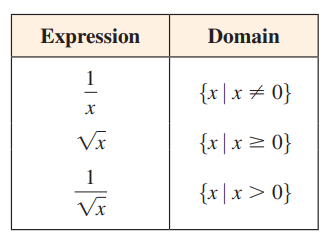
\includegraphics{algebra-pre-calculus/rational-expressions/expressions_domain.png}
\end{align*}

\subsection{Finding the Domain of an Expression}
Find the domains of the following expressions:
\textbf{(a)} $2x^2+3x-1$
This polynomial is defined for every x. Thus the domain is the set $\mathbb{R}$ of real
numbers. \\
\textbf{(b)} $\displaystyle \frac{x}{x^2-5x+6}$ \quad $\rightarrow$ We first factor the denominator. 
$$ x^2-5x+6 = (x-2)(x-3)$$ Since the denominator is zero when $x=2$ or $x=3$, the domain is the set of all real numbers except 2 and 3. So: $$ \text{Domain} = \{ x \in \mathbb{R} \mid x \neq 2, 3 \}$$
\\ \break 
\textbf{(c)} $\displaystyle \frac{\sqrt{x}}{x-5}$ \quad $\rightarrow$ For the numerator to b e defined, we must have $x\geq0$. Also we cannot we divide by zero, so $x\neq5$
Thus the domain is the set of all real numbers greater than or equal to zero, except 5. So: $$ \text{Domain} = \{ x \in \mathbb{R} \mid x \geq 0, x \neq 5 \}$$

\subsection{Simplifying Rational Expressions}
To \textbf{simplify rational expressions}, we factor both the numerator and the denominator and then \textbf{cancel} common factors from the numerator and denominator.
Like: $$ \frac{x^2-1}{x^2+x-2} = \frac{\cancel{(x-1)}(x+1)}{\cancel{(x-1)}(x-2)}=\frac{x+1}{x-2}$$


\subsection{Multiplying and Dividing Rational Expressions}
To \textbf{multiply rational expressions}, we are multiplying the numerators and denominators together. Like: $$ \frac{2x}{x^2-1} \cdot \frac{x^2-1}{x^2+1} = \frac{2x(x^2-1)}{(x^2-1)(x^2+1)} = \frac{2x}{x^2+1}$$ 

When it comes to \textbf{divide rational expressions}, we are multiplying the numerator by the reciprocal of the denominator. Like: $$ \frac{2x}{x^2-1} \div \frac{x^2-1}{x^2+1} = \frac{2x}{x^2-1} \cdot \frac{x^2+1}{x^2-1} = \frac{2x(x^2+1)}{(x^2-1)(x^2+1)} = \frac{2x}{x^2-1}$$

\subsection{Adding and Subtracting Rational Expressions}
To \textbf{add or subtract rational expressions}, we need to find a common denominator. We can do this by finding the least common multiple of the denominators. Like: $$ \frac{2}{x-1} + \frac{3}{x+1} = \frac{2(x+1)}{(x-1)(x+1)} + \frac{3(x-1)}{(x-1)(x+1)} = \frac{2x+2}{(x-1)(x+1)} + \frac{3x-3}{(x-1)(x+1)} = \frac{5x-1}{(x-1)(x+1)}$$

\subsection{Rationalizing the denominator or the Numerator}
If a fraction has a denominator of the form $A+B\sqrt{C}$, we can rationalize the denominator by multiplying numerator and denominator by the conjugate radical(its opposite) $A-B\sqrt{C}$.
This works because, by Special Product Formula 1, the product of the
denominator and its conjugate radical does not contain a radical:

$$ (A+B\sqrt{C})(A-B\sqrt{C})=A^2-B^2C$$

\subsection{Rationalizing the Denominator}
Rationalise the denominator: $\displaystyle \frac{1}{1+\sqrt{2}}$ \\ \break
We can multiply the numerator and denominator by the conjugate radical $1-\sqrt{2}$:
$$ \frac{1}{1+\sqrt{2}} \cdot \frac{1-\sqrt{2}}{1-\sqrt{2}} = \frac{1-\sqrt{2}}{1^2-(\sqrt{2})^2} = \frac{1-\sqrt{2}}{1-2} = \frac{1-\sqrt{2}}{-1} = \sqrt{2}-1$$
Here what we did is that we multiplied the numerator and denominator by the conjugate radical $1-\sqrt{2}$, then we simplified the denominator by using the Special Product Formula 1, and then we simplified the fraction.


\subsection{Rationalizing the Numerator}

Rationalise the numerator: $\displaystyle \frac{\sqrt{4+h}-2}{h}$ \\ \break
We can multiply the numerator and denominator by the conjugate radical $\sqrt{4+h}+2$:
$$ \frac{\sqrt{4+h}-2}{h} \cdot \frac{\sqrt{4+h}+2}{\sqrt{4+h}+2} = \frac{(\sqrt{4+h})^2-2^2}{h(\sqrt{4+h}+2)} = \frac{4+h-4}{h(\sqrt{4+h}+2)} = \frac{h}{h(\sqrt{4+h}+2)} = \frac{1}{\sqrt{4+h}+2}$$
Here what we did is that we multiplied the numerator and denominator by the conjugate radical $\sqrt{4+h}+2$, then we simplified the numerator by using the Special Product Formula 1, and then we simplified the fraction.


\subsection{Avoid Common Errors}
Don’t make the mistake of applying properties of multiplication to the operation of addition.
Many of the common errors in algebra involve doing just that. The following table states
several properties of multiplication and illustrates the error in applying them to addition.

\begin{align*}
    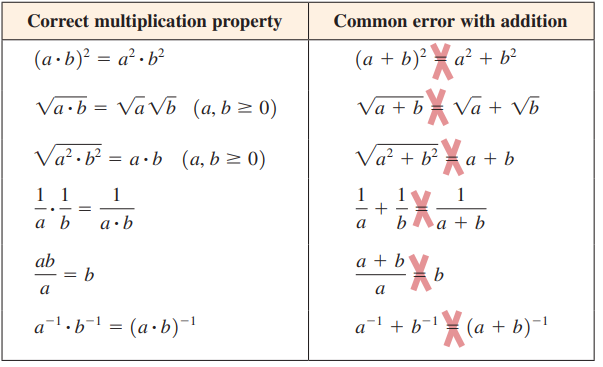
\includegraphics{algebra-pre-calculus/rational-expressions/common_errors.png}
\end{align*}

To verify that the equations in the right-hand column are wrong, simply substitute
numbers for a and b and calculate each side. % Section 5 - Rational Expressions
% Chapter 1 end - Algebra

% Chapter 2- Introduction to AI and ML %
\chapter{Introduction to AI and Machine Learning}
\section{Preface}
Anytime you see a computer do something that appears to be intelligent, like recognising a face, playing a game better than people can, driving cars these are all examples of artificial intelligence (AI). 
We will begin this chapter with search. Like we have an AI or some kind of program that can search to solutions to some kind of problem. Whether it is trying to figure out how to get from point A to point B or how to win a game.
After that we will take a look at knowledge. We want our AI to be able to represent knowledge and use that knowledge to make decisions. 
Then we will explore the topic of uncertainty. We will look at how we can represent uncertainty and how we can use that to make decisions. By extension we will also talk about probability, and how computers can deal with uncertainty to be more intelligent and rational.
After that we will turn out attention to optimization. We will look at how we can optimize a solution. Especially when there might be multiple ways of solving that problem, but we are looking for a better way, or potentially the best way possible to solve that problem.
Then we will look at learning and machine learning. Of how when we have access to data, our computers can be programmed to be quite intelligent by learning from data, and learning from experience.
We will also look at that how computers are able to draw inspiration from human intelligence, looking at the structure of a human brain, and how neural networks can be a computer analog of that.
Finally we will take a look at language and how computers can understand language, and how they can generate language. This what we call natural language processing. % Preface      
\end{document}